%%%%%%%%%%%%%%%%%%%%%%%%%%%%%%%%%%%%%%%%%%%%%%%%%%%%%%%%%%%%%%%%%%
%%%%%%%% CPSC 66 FALL 2025  REPORT %%%%%%%%%%%%%%%%%%%%%%%%
%%%%%%%% This template is modified from ICML 2014 %%%%%%%%%%%%%%%%
%%%%%%%%%%%%%%%%%%%%%%%%%%%%%%%%%%%%%%%%%%%%%%%%%%%%%%%%%%%%%%%%%%

\documentclass{article}

%include any external packages here.  This is similar to loading a
%library in python or C++

% use Times
\usepackage{times}
% For figures
\usepackage{graphicx}
\usepackage{subfigure}

% For citations
\usepackage{natbib}

% For algorithms and pseudocode
\usepackage{algorithm}
\usepackage{algorithmic}

%Adds hyperlinks to your citations automatically
\usepackage{hyperref}

% Packages hyperref and algorithmic misbehave sometimes.  We can fix
% this with the following command.
\newcommand{\theHalgorithm}{\arabic{algorithm}}

\usepackage[accepted]{icml2014}


% If your title is long (below), use this command to also provide
% short version.  This will go on the top of every page
\icmltitlerunning{Final Report}

\begin{document}

\twocolumn[ %use two column if you need a text to span across the whole page
\icmltitle{ CPSC 66 Final Report: \\ % \\ force a new line
Predicting NBA Lineup Efficiency Using Player Archetypes }

\icmlauthor{Jonathan Stump}{jstump2@swarthmore.edu}
\icmlauthor{Devin Burger}{dburger1@swarthmore.edu}
\icmlauthor{Lila Travers}{ltraver1@swarthmore.edu}
\icmlauthor{Sofie Aird}{saird1@swarthmore.edu}

\vskip 0.3in
]

\begin{abstract}
This project predicts the efficiency of NBA lineups based on combinations of player archetypes. 
We began by using PCA analysis and K-means++ to identify and define player archetypes within 
each basketball position. Once we have defined clusters from 2024-25 season statistics, these 
clusters enable us to label every player according to their attributes by more categories than 
traditional positions. We then used these labels to predict future lineup efficiency using season 
data to train and validate a Random Forest model capable of predicting lineup efficiency. Through 
our analysis we assessed whether player type and combinations of specific attributes can reveal 
the most efficient NBA lineup. This data-driven analysis reveals the player archetype combinations 
that will lead to success in the NBA.
\end{abstract}

\section{Introduction}
\label{introduction}

Traditional basketball analysis evaluates players and lineups using the five fixed positions and 
individual statistics. However, modern NBA success increasingly depends on how different player 
skill sets fit together, as lineups are more positionless and players contribute in diverse ways 
that traditional labels fail to capture. This project addresses the question: can player archetypes 
provide a predictive and interpretable representation of lineup efficiency and success?

To answer this, we designed a two-stage machine learning approach that combines multiple algorithms 
to model both player characteristics and lineup performance. First, we applied Principal Component 
Analysis and K-means clustering to identify player archetypes based on each player's individual 
statistics across the 2024-25 season. These archetypes capture meaningful playstyle differences 
among players, such as shooting, defensive impact, and rebounding. We then used these archetype 
combinations in a Random Forest Model trained on the 2024-25 lineup data to predict the PlusMinus 
statistic given a set of 5 players. We chose the PlusMinus statistic, which measures points scored 
minus points against, as the overall measure of efficiency and success of a team. 

By combining unsupervised and supervised machine learning techniques within a unified framework, 
this project illustrates how data-driven approaches can reveal meaningful structure in high-dimensional 
data.



\section{Methods}
\label{methods}

Our methodology includes three main strategies to make our data interpretable, and generalize 
trends to make accurate predictions. First, we used Principal Component Analysis (PCA) to reduce 
the dimensionality of our data. We then used K-Means clustering on our PCA-transformed data to 
identify player archetypes based on statistical profiles. Finally, after assigning each player 
to its clustered label, we trained a Random Forest model based on NBA lineups and their PlusMinus 
scores to generate future predictions of lineup effectiveness. 

For reference, we chose to predict the PlusMinus point differential compound statistic as our 
measure of success for a lineup. In this paper, efficiency refers to the PlusMinus statistic per 
100 possessions which is alternatively known as NetRtg (net rating)\footnote{“NBA Advanced Stats” NBA. Accessed December 14, 2025. https://www.nba.com/stats/help/glossary. }.

\subsection{Principal Component Analysis}
Because our player-level dataset contains a large number of correlated statistics, 
dimensionality reduction is a necessary preprocessing step prior to clustering. Reducing the 
dimensionality of our statistics was important to remove noise, minimize correlated statistics, 
and increase interpretability. We used Principal Component Analysis to understand how many 
dimensions were necessary while maintaining as much variance as possible. Given so many 
statistics from each game, play, and player, we wanted to make sure we were stripping out 
statistics that were correlated or unnecessary for clustering. Figure 1 depicts the variance 
from each principal component.

\begin{figure}[ht]
\vskip 0.1in
\begin{center}
\centerline{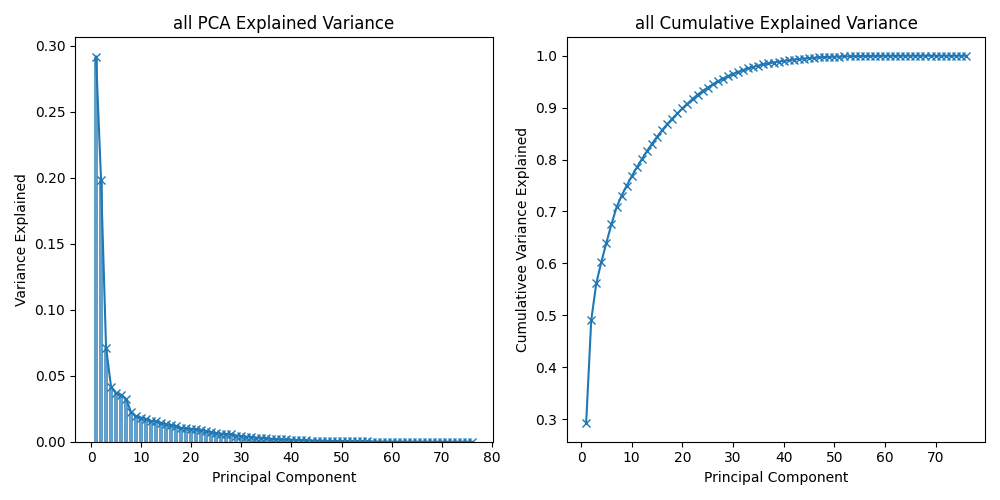
\includegraphics[width=\columnwidth]{all_pca_variance.png}}
\caption{This plot shows the proportion of variance explained by each principal component computed from player statistics across all positions. From this graph it is clear that around 9 principal components explain a majority of the variance in the data.}
\label{pcaPlot}
\end{center}
\vskip -0.2in
\end{figure}

Figure 1 above shows the PCA for all positions, but it is important to note we ran PCA 
separated by position before clustering. Because player statistics differ substantially across 
positions, we perform PCA separately for each position group to ensure that dominant sources of
 variance reflect role-specific patterns specific to each position. The resulting components 
 are then used for visualization and clustering within each position. Finally, we used PCA to 
 increase interpretability. As shown in Figure 2, we wanted to be able to visualize the clusters 
 and the groups of players that are similar. From reducing dimensionality, we were then able to 
 visualize the clusters more easily in two dimensions.

 Finally, we used PCA to increase interpretability. As shown in Figure 2 we wanted to be able to 
 visualize the clusters and the groups of players that are similar. From reducing dimensionality, 
 we were then able to visualize the clusters more easily in two dimensions.


\begin{figure}[ht]
\vskip 0.1in
\begin{center}
\centerline{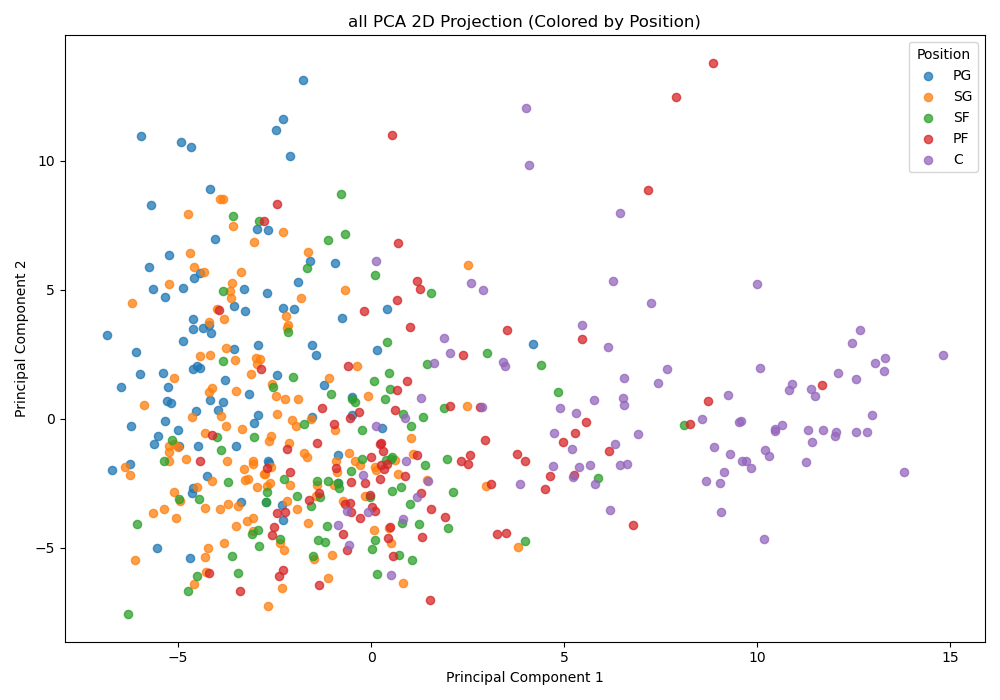
\includegraphics[width=\columnwidth]{all_pca_2d_by_position.png}}
\caption{This plot shows all players represented in the first two principal components computed from player statistics across all positions. Each position is color coded}
\label{pcaPlot}
\end{center}
\vskip -0.2in
\end{figure}



\subsection{K-Means Clustering}
After using PCA to reduce dimensionality, our main method was to use K-Means to cluster the players into archetypes 
based on their statistics. We used the gap statistic to determine the optimal k on a per-player basis, as this statistic 
values a stronger clustering structure compared to random data. More specifically, the gap statistic measures how much
 better the observed clustering compactness is compared to what would be expected under a null reference distribution with 
 no inherent cluster structure. Typical methodology using the gap statistic suggests 
choosing k such that the gap statistic of $k+1$ clusters is not significantly better than k clusters, as the gap statistic 
generally rises with k. We found that this k was too small for our clusters to be interpretable, so we averaged this 
k with the k matching the highest gap statistic for all k less than or equal to ten, our assumption being more than ten 
archetypes per position is too specific to capture trends with limited lineup data.


\begin{figure}[ht]
    \vskip 0.1in
    \begin{center}
    \centerline{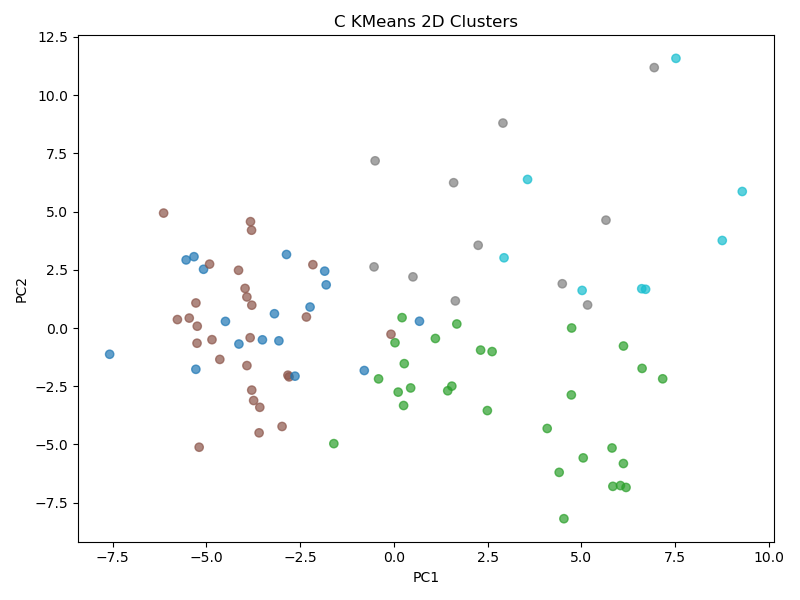
\includegraphics[width=\columnwidth]{C_kmeans5.png}}
    \caption{This plot shows the clustering result for the Center position, as represented in two dimensions}
    \label{pcaPlot}
    \end{center}
    \vskip -0.2in
\end{figure}

To ensure these clusters were interpretable, we printed the top ten players closest to the cluster centers. 
In addition, checking the statistical features that differ most from one cluster to the others in that position 
provided insight into why those players were clustered together. This was done by taking the difference between the 
standardized statistics for the players in a singular cluster and the mean standardized statistics of the other clusters 
in a particular position, and seeing which statistical features differed most from the mean in magnitude. Most 
clusters were defined by one particular skill – such as rebounding or three point shooting – but other clusters outlined 
players traditionally seen as ‘better’ than others – high points and usage relative to the mean – or ‘worse’ than others 
– low shooting percentage, defensive rating, etc. For more in depth analysis on the interpretability of the clusters, 
see the results section.


\subsection{Random Forest Model}
To evaluate whether player archetypes contain predictive signals for lineup performance, we employed 
a Random Forest regression model to predict lineup efficiency from archetype composition. Random 
Forests are ensemble learning methods that combine the predictions of multiple decision trees, each 
trained on a different bootstrap sample of the data. We believe Random Forest regression is 
well-suited to this task for several reasons. First, lineup performance may depend on nonlinear 
interactions between player types that are difficult to capture with linear models. Bootstrapped 
decision trees naturally model these complex interactions, and the ensemble structure of Random 
Forests reduces overfitting while maintaining flexibility. Second, Random Forests require minimal 
feature engineering and are robust to noisy or weakly informative features, which is important 
given the variability in predicting lineup efficiency. 

Each lineup was represented as a fixed-length feature vector representing the archetypes of the 
players in the lineup. Because NBA lineups often do not have one of each position on the floor 
at the same time, we adopted a one-vs-all representation in which each feature corresponds to 
one player archetype, rather than having five features representing the archetype of a specific 
position. The value of each feature indicates the number of players from that archetype present 
in the lineup. This approach allows the model to accommodate lineups with unconventional 
positional configurations, such as multiple guards or positionless lineups, without imposing 
artificial constraints.

In total, each observation consisted of 25 archetype count features, corresponding to the 
clusters identified across all positions. Lineup minutes played were not included as a predictive 
feature but were instead used as sample weights during training and evaluation, ensuring that 
lineups appearing more frequently in games contributed proportionally to the learning objective. 
The target variable was the lineup’s efficiency rating.

We trained the Random Forest model using scikit-learn’s RandomForestRegressor. Model performance 
was evaluated using five-fold cross-validation, with each fold preserving the full distribution 
of lineup observations. Within each training fold, hyperparameters were tuned using grid search 
to identify configurations that maximized predictive performance. The hyperparameters considered 
included the maximum depth of each tree, the number of features considered at each split, 
the minimum number of samples required at leaf nodes, and the total number of trees in the 
ensemble.

For each cross-validation fold:
\begin{itemize}
    \item The model was trained on 80\% of the data, with lineup minutes used as sample weights.
    \item Tune hyperparameters via grid search
    \item Evaluate weighted R² on held-out fold
    \item Aggregate performance across folds
\end{itemize}



\subsection{Analysis of Methods}
We employed clustering to identify patterns in player types from statistics to move beyond traditional 
position categorization. By grouping players with similar statistical profiles into archetypes, PCA 
and K-Means clustering provides an interpretable representation of player roles such that we can identify
the most effective skill sets for on-court performance. In particular, clustering exposes statistical 
dimensions that most differentiate player roles. This abstraction aligns with important considerations 
of coaches when constructing lineups. It is important to consider complimentary roles and skills when 
laying out a team.

We chose the Random Forest model because it can capture complex, nonlinear interactions between player 
archetypes that influence lineup performance. The ensemble nature of Random Forests reduces overfitting while
maintaining flexibility to model complex data.


\section{Experiments and Results}
\label{results}
\subsection{Data Collection and Preprocessing}
We used two distinct NBA datasets aggregated from official NBA box scores and play-by-play data. 
The first dataset, \textbf{NBA Player Stats: Per 100 Possessions (2024-25, 2025-26)}, contains season-level 
individual player statistics and is used to identify player archetypes. The second dataset, \textbf{PBP 
NBA Lineup Stats (2024-25, 2025-26)}, contains season-level statistics for five-man lineups and is 
used to model lineup efficiency. What we are referring to as overall team efficiency is also 
known as “PlusMinus.” PlusMinus is a composite statistic that subtracts points against from points 
for during the time that any given lineup is on the court. This values the strength of a lineup, 
and to predict a lineup's PlusMinus output will give us valuable insight into the future success 
of a team. 

All analysis was conducted using Python, with sci-kit learn libraries for preprocessing, 
clustering, and modeling. Prior to analysis, we applied several preprocessing steps to ensure the 
data was consistent and interpretable. First, player and lineup features were measured on different 
scales, with some recorded as raw counts and others as percentages. To prevent scale-driven bias, 
all numerical features were standardized. Second, the individual player dataset included full names, 
while the lineup dataset listed only last names, preventing direct alignment between the two. 
We addressed this by writing a Python script to match last names to full player names, enabling 
consistent player identification and allowing archetype labels to be correctly assigned to each 
five-man lineup. Finally, we removed overly specific and redundant features, such as highly 
granular shot-type statistics, to reduce noise, improve computational efficiency, and increase 
model stability. These steps helped ensure our analysis reflected real player roles and lineup 
behavior, not distortions caused by data formatting or scale

\subsection{Clustering Results}
To interpret the resulting player archetypes, we examined each cluster by identifying 
(1) the number of clusters and the amount of players per cluster 
(2) the players closest to the cluster centroid and 
(3) the statistics that most strongly differentiated each cluster from the others. 
Positive values indicate features that are more associated within a cluster, 
while negative values indicate features that are less associated relative to 
other clusters. 

As an example, we consider the point guard (PG) position, for which four 
distinct clusters were identified, with the following sizes:
\begin{itemize}
    \item Cluster 0: 34 players
    \item Cluster 1: 28 players
    \item Cluster 2: 22 players
    \item Cluster 3: 16 players
\end{itemize}

Table \ref{tab:pg_cluster0} summarizes the characteristics of Point Guard Cluster 0. Table \ref{tab:pg_cluster1}
summarizes the characteristics of Point Guard Cluster 1.
We will interpret these two clusters' characteristics as an example of the value of our 
clustering approach. 

\begin{table}[t]
\centering
\small
\caption{Summary of Point Guard Cluster 0 archetype characteristics.}
\label{tab:pg_cluster0}
\begin{tabular}{p{2cm} p{4.5cm}}
\hline
\textbf{Attribute} & \textbf{Cluster 0 (PG)} \\ 
\hline \\

Number of Players & 34 \\

Representative Players & Reggie Jackson, Mike Conley, Jose Alvarado, Aaron Holiday, 
Marcus Smart, Cameron Payne, Marcus Sasser, Keaton Wallace, Mont\'e Morris, Fred VanVleet 
\\

Dominant Positive Features &  FG3APct  ($+1.96$) \newline
 AtRimFG3AFrequency ($+1.82$)\newline
  PtsAssisted3s ($+1.73$) 
  \\

Dominant Negative Features &  ShortMidRangeFrequency ($-1.97$)\newline
 AtRimFGA ($-1.87$) \newline
PtsAssisted2s ($-1.86$) \newline
DefThreePtReboundPct ($-1.68$) \newline
PtsPutbacks ($-1.66$) 
\\

Archetype Interpretation & Perimeter-oriented point guards emphasizing three-point 
shooting and assisted perimeter scoring, with limited rim pressure and rebounding contribution 
\\ 

\hline
\end{tabular}
\end{table}

\begin{table}[t]
\centering
\small
\caption{Summary of Point Guard Cluster 1 archetype characteristics.}
\label{tab:pg_cluster1}
\begin{tabular}{p{2cm} p{4.5cm}}
\hline
\textbf{Attribute} & \textbf{Cluster 1 (PG)} \\ 
\hline \\

Number of Players & 23 \\

Representative Players &   Anthony Black, Killian Hayes, Devin Carter, Terry Rozier, Jrue Holiday, 
Bruce Brown, KJ Simpson, Craig Porter Jr., Scotty Pippen Jr., Kris Dunn \\

Dominant Positive Features &  OffRebounds                 (+1.99) \newline
OffFGReboundPct             (+1.99) \newline
OffThreePtReboundPct        (+1.99)\newline
OffThreePtRebounds          (+1.98) \newline
ShotQualityAvg              (+1.93) \newline \\

Dominant Negative Features &  LongMidRangeAccuracy       (-1.96) \newline
NonHeaveFg3Pct             (-1.93) \newline 
Avg2ptShotDistance         (-1.93) \newline
UnblockedCorner3Accuracy(-1.90) \newline
Corner3Accuracy            (-1.89) \newline \\

Archetype Interpretation & Rebounding-focused players who generate value through offensive boards and 
high-quality shots near the basket. These players are bigger, more physical guards who are known 
for their athleticism. \\ 

\hline
\end{tabular}
\end{table}

These features suggest that Cluster 0 is characterized by point guards who rely heavily on 
three-point shooting, as evidenced by elevated three-point attempt percentage and assisted 
three-point scoring. Conversely, players in this cluster tend to take fewer shots at the rim, 
generate fewer assisted two-point baskets, and contribute less to rebounding and putback scoring. 
This interpretation is reinforced by the players nearest to the cluster centroid, who are 
predominantly smaller, perimeter-oriented guards. While many of these players are capable shooters, 
they generally do not score across a wide variety of locations, instead specializing in 
perimeter-based roles.

Point Guards in cluster 1 contribute significantly to rebounding, shooting poorly from behind the 
three point line and taking less shots from long distances. Instead, these guards shoot high 
quality shots from short range and grab offensive rebounds. This is supported by the players 
closest to the cluster center – mostly taller and guards who use their strength, speed, or vertical 
jump to get close to the basket. It’s easy to see that though these players play the same 
position as those in PG Cluster 0, these are two vastly different styles of play.

Not just for Point Guards, but across all 25 clusters spanning the five positions, we found that each cluster was highly 
interpretable and exhibited clear stylistic distinctions. Several clusters aligned closely 
with well-established basketball archetypes. For example, Center Cluster 3 consisted primarily 
of tall, athletic centers who specialized in rim protection and finishing efficiently near the 
basket. Shooting Guard Cluster 0 was defined by players who emphasized three-point shooting and perimeter 
defense, reflecting a classic “3-and-D” role. Small Forward Cluster 2 captured larger 
wings who prioritized attacking the rim and generating offense through drives rather than perimeter 
shooting. Finally, Power Forward Cluster 4 was composed of smaller, floor-spacing forwards
 who frequently operated from the corners and stretched opposing defenses with their three-point 
 shooting.

Notably, for every position, at least one cluster consisted primarily of elite, high-usage 
players. (EX PF Cluster 0: Paolo Banchero, Scottie Barnes, Paul George, Kevin Durant, Jayson Tatum) 
Clusters of this type were consistently differentiated from other clusters by substantially 
higher scoring-related statistics. The emergence of such clusters provides additional 
validation that the clustering approach successfully captured meaningful differences in 
player roles and performance profiles.

To support this assertion, we calculated the average PlusMinus for each cluster to gain insight
 into archetypes that have significantly positive or negative effects on lineup performance. 
 Unsurprisingly, clusters that included elite, high-usage players were in the positives, but 
 some archetypes that had flown under radar were shown to contribute significantly to efficient 
 lineups. For example, Centers that spaced the floor by shooting from the perimeter, and 
 particularly the corner (Center cluster 1), had the highest average PlusMinus across lineups 
 with 7.42. One possible reason for this may be that spot-up shooting Centers open up space for 
 other players to cut and drive to the basket, raising the effectiveness of other players in 
 their lineups. This affirmed our belief that there are underlying relationships between 
 archetypes that contribute to lineup efficiency, relationships we hoped to be capturable 
 through certain regression models. 

To further see effects on lineup efficiency by individual clusters, we trained a linear regression 
model and examined the learned coefficients. While the linear regression model performed worse 
than the Random Forest, the coefficients provide a direct interpretation of archetype contributions 
to lineup efficiency, representing the marginal change in lineup PlusMinus (per 100 possessions) 
associated with adding one additional player from a given positional cluster and holding the 
rest of the lineup composition fixed. Interestingly, Center cluster 1 had the fifth highest 
coefficient of 2.99, with the highest coefficient (4.99) belonging to Center cluster 4 – Centers 
who scored a lot from the perimeter and free throw line but also achieved a high number of assists. 
One unexpected result was Shooting Guard cluster 3 – a cluster of guards different from other 
archetypes by their rebounding on both ends of the floor – which achieved the second highest 
weighted average PlusMinus (6.99) and second highest learned coefficient (4.94). This is surprising, 
as rebounding isn’t typically considered a high priority for Shooting Guards, suggesting this trait 
may be undervalued for the position. 



\subsection{Random Forest Results}
Across cross-validation folds on the 2024–25 data, the archetype-based Random Forest achieved a mean 
weighted R² of 0.11 (standard deviation 0.06). The R² metric shows the proportion of the variance in 
our PlusMinus label that can be explained by the cluster features. A low R² indicates that the model 
does not fit the data well, and does not perform significantly better than predicting the mean 
PlusMinus. While predictive performance varied across folds, an R² of 0.11 demonstrates that the 
model consistently explained a non-trivial portion of variance in lineup efficiency relative to a 
constant baseline. The Random Forest also achieved a mean weighted mean squared error (MSE) of 
213.6 (standard deviation 23.3). This corresponds to an average root mean squared error of approximately 
14.6 points per 100 possessions, meaning our efficiency predictions were off by roughly this estimate. 

When the same model was applied to 2025–26 lineups, performance deteriorated substantially. Cross-season 
evaluation yielded a negative weighted R² (−0.02) and a mean weighted MSE of 725.9 (standard deviation 183.5), 
corresponding to a root mean squared error of roughly 27.0 points per 100 possessions. Despite 
attempts to constrain model complexity by limiting tree depth and increasing the minimum number 
of samples per leaf, we were unable to increase the 2025–26 R² beyond 0.02. These results indicate 
limited generalization across seasons when using archetype-based Random Forest predictions, suggesting 
that lineup efficiency is influenced by substantial season-specific factors not captured by archetype 
composition alone.


To investigate whether information loss from dimensionality reduction and clustering contributed 
to the limited predictive performance, we conducted a parallel experiment using raw player 
statistics rather than archetypes. In this setting, each player in a lineup was represented 
using a reduced set of 15 per-100-possession statistics selected to balance expressiveness and 
redundancy. Lineup feature vectors were constructed by concatenating individual player statistics, 
and the same Random Forest training and evaluation procedure was applied.

The raw-statistics model achieved a mean weighted R² of 0.08 during cross-validation on 2024–25 
data, comparable to the archetype-based model. When applied to 2025–26 lineups, the raw-statistics 
model achieved a barely positive weighted R² (0.03) and higher weighted correlation (0.24) 
relative to the archetype-based approach, though overall predictive performance remained limited.

Together, these results suggest that neither archetype-based and raw-statistic Random Forest 
approaches generalizes strongly across seasons. Importantly, the comparable performance of the 
two models indicates that clustering and dimensionality reduction did not result in substantial 
information loss. Instead, the limited predictive accuracy likely reflects the complexity of 
predicting lineup efficiency, which is influenced in significantly more ways than the player’s 
play styles or stats.


\section{Social Implications and Discussion}
\label{Social Implications}

The key stakeholders in this project include NBA coaches, front-office decision makers, 
players, and fans and media analysts. Coaches and analytics staff stand to benefit directly 
from clearer insights into player archetypes and lineup efficiency, which can support decisions 
around rotations, roster construction, and mid-game adjustments. Front offices may use these 
results to inform drafting, trades, and contract valuation by identifying undervalued and 
overvalued skill combinations, as well as complementary player profiles. Players could benefit 
if the analysis highlights the value of subjective and off-ball impact, but they could also be 
disadvantaged if metrics or outputs oversimplify their role. Fans and media analysts may gain 
a deeper understanding of why certain lineups succeed and may see their favorite team succeed 
because of these analyses, though there is also a risk of overemphasizing styles of play approved 
by the model at the expense of creativity or team identity.

This work interacts with existing power dynamics by potentially shifting influence further 
toward data and analytics within basketball organizations, which may empower analytically 
inclined staff while marginalizing experiential knowledge from coaches or scouts if used 
uncritically. There are also real concerns about misuse: models trained on historical data may 
reinforce existing biases (e.g., undervaluing certain positions, play styles, or players with 
smaller sample sizes) and if model outputs are treated as definitive causal claims rather than 
decision-support signals with uncertainty, they can lead to overconfidence, misallocation of 
playing time or salary, and unfair evaluations of players

From an economic and ethical perspective, these models could influence salaries, playing time, 
and career longevity, raising questions about transparency, accountability, and fairness. Rather 
than serving as a definitive decision-maker, this project is best viewed as a decision-support 
tool whose value depends on careful integration with domain expertise, awareness of limitations, 
and ongoing evaluation of how its outputs affect both competitive balance and individual 
stakeholders.



\section{Conclusions}
\label{conclusion}

Despite limited predictive performance, one of the most compelling outcomes of this work was 
the interpretability of the learned archetypes. The clustering approach consistently produced 
intuitive groupings in ways that could be useful for similar projects looking to evaluate player 
archetypes.

This project does yield questions and future work. First, incorporating contextual information 
such as opponent lineups, game state, or possession-level data could improve predictive performance 
by capturing factors that strongly influence lineup outcomes. Second, more complex models 
like neural networks or more advanced architectures beyond the scope of this class may better 
capture some of the nonlinear relationships between players. It is important to note though, 
that such approaches may come at the cost of interpretability. Overall, this project demonstrates 
both the strengths and limitations of archetype-based modeling for lineup analysis.


\section*{Acknowledgments}

We would like to thank Professor Gabriel Hope for his support throughout the work for this 
paper. We would also like to acknowledge the help provided by student feedback from our peers. 
Thank you to those who provided helpful comments during the last stages of our work. Our work
is supported by the Swarthmore College Computer Science department. 

% In the unusual situation where you want a paper to appear in the
% references without citing it in the main text, use \nocite

\nocite{*}

\bibliography{references}
\bibliographystyle{icml2014}

\end{document}


% This document was modified from the file originally made available by
% Pat Langley and Andrea Danyluk for ICML-2K. This version was
% created by Lise Getoor and Tobias Scheffer, it was slightly modified
% from the 2010 version by Thorsten Joachims & Johannes Fuernkranz,
% slightly modified from the 2009 version by Kiri Wagstaff and
% Sam Roweis's 2008 version, which is slightly modified from
% Prasad Tadepalli's 2007 version which is a lightly
% changed version of the previous year's version by Andrew Moore,
% which was in turn edited from those of Kristian Kersting and
% Codrina Lauth. Alex Smola contributed to the algorithmic style files.
